\documentclass{article}

% if you need to pass options to natbib, use, e.g.:
% \PassOptionsToPackage{numbers, compress}{natbib}
% before loading nips_2016
%
% to avoid loading the natbib package, add option nonatbib:
% \usepackage[nonatbib]{nips_2016}

\usepackage{nips_2016}

% to compile a camera-ready version, add the [final] option, e.g.:
%\usepackage[final]{nips_2016}

\usepackage[utf8]{inputenc} % allow utf-8 input
\usepackage[T1]{fontenc}    % use 8-bit T1 fonts
\usepackage{hyperref}       % hyperlinks
\usepackage{url}            % simple URL typesetting
\usepackage{booktabs}       % professional-quality tables
\usepackage{amsfonts}       % blackboard math symbols
\usepackage{nicefrac}       % compact symbols for 1/2, etc.
\usepackage{microtype}      % microtypography

\title{Deep Models for Ensemble Improvisation}

% The \author macro works with any number of authors. There are two
% commands used to separate the names and addresses of multiple
% authors: \And and \AND.
%
% Using \And between authors leaves it to LaTeX to determine where to
% break the lines. Using \AND forces a line break at that point. So,
% if LaTeX puts 3 of 4 authors names on the first line, and the last
% on the second line, try using \AND instead of \And before the third
% author name.

\author{
  Charles P. Martin\thanks{\url{http://charlesmartin.com.au}}\\
  Department of Informatics\\
  University of Oslo\\
  Norway\\
  \texttt{charlepm@ifi.uio.no}\\
  %% examples of more authors
  %% \And
  %% Coauthor \\
  %% Affiliation \\
  %% Address \\
  %% \texttt{email} \\
  %% \AND
  %% Coauthor \\
  %% Affiliation \\
  %% Address \\
  %% \texttt{email} \\
  %% \And
  %% Coauthor \\
  %% Affiliation \\
  %% Address \\
  %% \texttt{email} \\
  %% \And
  %% Coauthor \\
  %% Affiliation \\
  %% Address \\
  %% \texttt{email} \\
}

\begin{document}

\maketitle

\begin{abstract}
  For many of us, the pursuit and enjoyment of musical performance
  goes hand-in-hand with collaborative creativity, whether in an
  choir, jazz combo, orchestra, or rock band. However, few musical
  interfaces use the affordances of computers to create or enhance 
  ensemble musical experiences.
  One possibility for such a system would be to use an artificial
  neural network to model the way other musicians respond to single
  performer. Some forms of music have well-understood rules for
  interaction; however, this is not the case for free improvisation
  with new touch-screen instruments where styles of interaction may be
  discovered in each new performance.
  This paper describes work-in-progress towards an ANN model of
  ensemble interactions that took place in such performances.
  Potential models have been trained on a corpus of ensemble
  touch-screen improvisations that has been made available from
  previous work. The motivations for creating these models will be
  explored, and the work so far will be evaluated by comparison with
  traditional Markov models and examination of the results.
\end{abstract}

\section{Improvising on Touch-Screens}



\begin{figure}
  \centering
  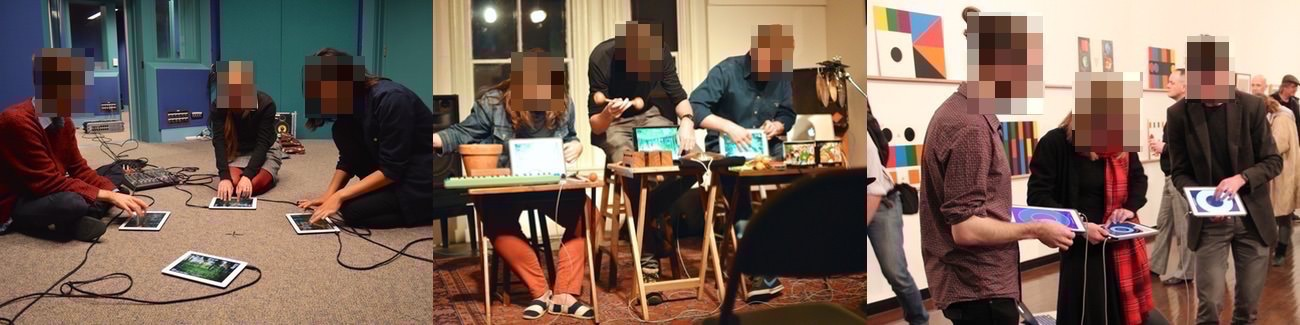
\includegraphics[width=\textwidth]{three-performance-contexts}
  \caption{In previous work, data was collected from more than 150
    collaborative interaction sessions including rehearsals,
    performances, installations, and demonstrations. This corpus
    constitutes a significant dataset for further investigations of
    creative interaction.}\label{fig:performance-contexts}
\end{figure}




\subsection{Interpreting Touch Data}



\subsection{Why model the ensemble?}




\section{An LSTM Model for Ensemble Performances}



\section{Evaluation of Results So Far}

\section{Conclusions and Future Work}





\subsubsection*{Acknowledgments}
This work is partially supported by The Research Council of Norway as
a part of the Engineering Predictability with Embodied Cognition
(EPEC) project, under grant agreement 240862.



\bibliographystyle{SIGCHI-Reference-Format}
\bibliography{2013ComputerMusic}

\end{document}
